%!TEX root = ../dokumentation.tex
\chapter{Datenbank}

\section{Hosting}
Zum Hosten der Datenbank wird die \href{https://aws.amazon.com/de/rds/mariadb/}{Amazon RDS for MariaDB} mit der MariaDB Version 10.2.21 verwendet. \\
\glqq\href{https://aws.amazon.com/de/rds/}{Amazon Relational Database Service (Amazon RDS)} ist ein Webservice, der das Einrichten, Betreiben und Skalieren einer relationalen Datenbank in der AWS Cloud vereinfacht.\grqq \cite{AmazonRDS} Amazon RDS unterstützt bis zu sechs verschiedene Datenbank-Engines, z.B. MySQL, PostgreSQL oder auch MariaDB. \cite{AmazonRDS}

Der Vorteil einer Cloud-basierten Datenbank ist, dass jeder Entwickler problemlos darauf zugreifen kann.\\
Um auf diese Datenbank zugreifen zu können, unterstützt AWS sogenannte Security Groups. Diese Gruppen dienen als virtuelle Firewall. Man bindet sie einer Ressource wie z.B. der Datenbank oder dem Elastic Beanstalk Server zu. In einer Security Group wird spezifiziert welche IPs und sonstige Ressourcen Zugriff haben.\\
Da während der Entwicklungszeit die IP Adresse von Luca sich ständig geändert hat, haben wir von überall Zugriff erlaubt. Dies stellt natürlich ein erhöhtes Sicherheitsrisiko dar, dennoch braucht man Anmeldedaten für die Datenbank. Nach der Entwicklungsphase wurde dieser Zugang entfernt.

\section{Verwendung von \$\_SERVER}
Damit die Anmeldedaten für die Datenbank nicht blank im Quellcode zu finden sind, wurden diese in dem \$\_SERVER Array des Webservers gespeichert. Dieses Verfahren wurde gewählt, da ein öffentliches Github Repository erstellt wurde und somit sonst für jeden sichtbar wäre.

Um die Daten auf dem lokalen Xampp Server verwenden zu können, werden diese in der \lstinline{httpd-xampp.conf} gespeichert. Im folgenden Codeblock werden die Anmeldedaten im Modul \lstinline{env\_module} definiert.

\begin{lstlisting}[language=bash]
#
# XAMPP settings
#

<IfModule env_module>
    ...
    SetEnv RDS_DB_NAME "planning_poker"
    SetEnv RDS_HOSTNAME "planning-poker.cztpemauxamy.eu-central-1.rds.amazonaws.com"
    SetEnv RDS_PASSWORD "<password>"
    SetEnv RDS_PORT "3306"
    SetEnv RDS_USERNAME "admin"
</IfModule>
\end{lstlisting}

Nun kann man innerhalb des Programmcodes auf das \$\_SERVER Array zugreifen um die zuvor definierten Werte aufzurufen. Dieser Codeblock, aus der Datei Model/ModelBase.php, zeigt die Funktion zur Erstellung der Datenbankverbindung. 

\begin{lstlisting}[language=PHP]
/**
* GetPDO: returns a PDO Connection
* @author Luca Stanger
* @return Database
*/
public function getPdo()
{
	if (self::$_db === null) {
		self::$_db = new \PlanningPoker\Model\Database(
			$_SERVER['RDS_HOSTNAME'],
			$_SERVER['RDS_PORT'],
			$_SERVER['RDS_DB_NAME'],
			$_SERVER['RDS_USERNAME'],
			$_SERVER['RDS_PASSWORD'],
			'utf8'
		);
	}

	return self::$_db;
}
\end{lstlisting}

Damit der AWS Elastic Beanstalk Server ebenfalls auf die Daten über \$\_SERVER zugreifen kann, werden diese unter den Konfigurationseinstellung in AWS als Umgebungseigenschaften definiert.

\section{Schema}
In der Abbildung \ref{datenbank} ist das Schema der Datenbank zu sehen.

\begin{figure}[H]
	\centering
  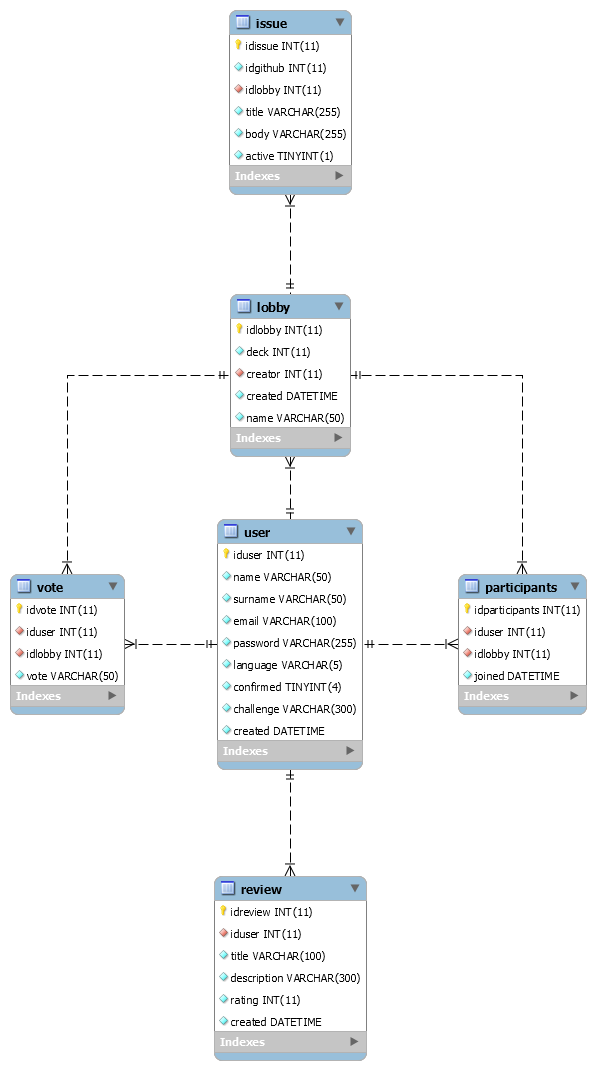
\includegraphics[width=0.8\textwidth]{images/database.png}
	\caption{Visualisierung der Datenbank}
	\label{datenbank}
\end{figure}

Zu sehen sind die einzelnen Tabellen der Datenbank mit Verknüpfungen zu anderen Tabellen. In einer Tabelle sind die einzelnen Spalten beschrieben. Primärschlüssel haben einen goldenen Schlüssel, Fremdschlüssel eine rote Raute und normale Spalten eine blaue Raute. Außerdem werden die Typen der Spalten gezeigt. Alle Verbindungen beschreiben eine 1:N Beziehung und die Cascade Regel.\\
Dadurch, dass alle Fremdschlüssel mit der Option ON DELETE CASCADE beschrieben werden, 
Ein Beispiel wäre: Ein User kann mehrere Lobbies als Ersteller besitzten, ein Vote in einer Lobby besitzten, aber mehrere Votes in mehreren Lobbies, er kann durch die Tabelle participants an mehrere Lobbies teilnehmen, aber jeweils nur einmal in einer Lobby teilnehmen und er kann mehrere Reviews schreiben.\\

Der Vorteil durch dieses Schema ist, wenn z.B. ein Benutzer gelöscht wird werden automatisch alle Daten dieses Benutzers aus den Verbunden Tabellen gelöscht. D.h. die Reviews, Lobbies die der Benutzer erstellt hat, die Teilnahme aus anderen Lobbies, sowie alle Votes aus den Lobbies werden gelöscht. Außerdem, weil die Lobbies des Benutzers gelöscht werden, werden auch die Issues dieser Lobby gelöscht.